\documentclass[11pt,a4paper]{article}
\usepackage[margin=23mm]{geometry}
\usepackage{amsmath}
\usepackage{booktabs}
\usepackage{graphicx}
\usepackage{float}
\usepackage{microtype}
\usepackage{multicol}
\usepackage[table]{xcolor}
\usepackage[hidelinks]{hyperref}

\setlength{\parindent}{0pt}
\setlength{\parskip}{0.55em}
\setlength{\columnsep}{1.2em}
\setlength{\multicolsep}{0.4em}
\raggedcolumns
\newcommand{\solverGT}{\textsc{Solver(GT)}}
\newcommand{\solverConvex}{\textsc{Convex Solver}}
\newcommand{\patchitem}[1]{\noindent\texttt{\detokenize{#1}}\par}

\title{Classification of the 100 Benchmark Patches by Solver-RMSE Ratio}
\author{}
\date{}

\begin{document}
\maketitle

\section{Criterion and counts}

For each patch $P$ with $N_P$ pixels, define the two whole-patch root mean square errors
\begin{align}
d_{\solverGT}(P)
  &= \sqrt{\frac{1}{N_P}\sum_{p=1}^{N_P}
      \left(\widehat{R}_{P,\solverGT}(p)-R_P(p)\right)^2},\\
d_{\solverConvex}(P)
  &= \sqrt{\frac{1}{N_P}\sum_{p=1}^{N_P}
      \left(\widehat{R}_{P,\solverConvex}(p)-R_P(p)\right)^2}.
\end{align}
The classification ratio is
\begin{equation}
q(P)=\frac{d_{\solverConvex}(P)}{d_{\solverGT}(P)}.
\end{equation}
A patch belongs to \textbf{Case 1} when $q(P)\geq 2$: the Convex Solver's RMSE is at least twice the RMSE of \solverGT, so \solverGT\ is much closer to the ground truth. A patch belongs to \textbf{Case 2} when $q(P)<2$: the two RMSE values are comparatively close. The equality is assigned to Case 1 by definition.

Applying this rule to all 100 patches gives
\begin{center}
\begin{tabular}{lrr}
\toprule
Classification & Number of patches & Percentage \\
\midrule
Case 1 ($q\geq 2$) & 24 & 24.0\% \\
Case 2 ($q<2$) & 76 & 76.0\% \\
\midrule
Total & 100 & 100.0\% \\
\bottomrule
\end{tabular}
\end{center}

The observed ratios range from 0.9846 to 11.7670. There is no patch in the interval between the largest Case 2 ratio (1.9767) and the smallest Case 1 ratio (2.6310).

\section{Distribution of the ratio}

Table~\ref{tab:ratio-distribution} reports the distribution of $q(P)$ across all 100 patches, independently of the assigned case. The intervals have width one and are left-closed and right-open.

\begin{table}[H]
\centering
\begin{tabular}{crr}
\toprule
Ratio interval & Number of patches & Percentage \\
\midrule
$[0,1)$ & 11 & 11.0\% \\
$[1,2)$ & 65 & 65.0\% \\
$[2,3)$ & 1 & 1.0\% \\
$[3,4)$ & 4 & 4.0\% \\
$[4,5)$ & 5 & 5.0\% \\
$[5,6)$ & 2 & 2.0\% \\
$[6,7)$ & 4 & 4.0\% \\
$[7,8)$ & 1 & 1.0\% \\
$[8,9)$ & 1 & 1.0\% \\
$[9,10)$ & 1 & 1.0\% \\
$[10,11)$ & 2 & 2.0\% \\
$[11,12)$ & 3 & 3.0\% \\
\midrule
Total & 100 & 100.0\% \\
\bottomrule
\end{tabular}
\caption{Distribution of $d_{\solverConvex}/d_{\solverGT}$ in bins of width one.}
\label{tab:ratio-distribution}
\end{table}

\section{Patch assignments}

The common identifier prefix \texttt{RAD\_OPERA\_HOURLY\_RAINFALL\_ACCUMULATION\_} is omitted below.

\subsection{Case 1: 24 patches}
\begin{multicols}{2}
\scriptsize
\setlength{\parskip}{0.18em}
\patchitem{202301190300_patch001}
\patchitem{202301210300_patch000}
\patchitem{202301210800_patch002}
\patchitem{202301210900_patch000}
\patchitem{202301211800_patch000}
\patchitem{202301211900_patch000}
\patchitem{202301211900_patch001}
\patchitem{202301222100_patch000}
\patchitem{202301230100_patch000}
\patchitem{202301231300_patch001}
\patchitem{202301240500_patch000}
\patchitem{202301241500_patch000}
\patchitem{202301241700_patch000}
\patchitem{202301241700_patch002}
\patchitem{202301242200_patch001}
\patchitem{202301250200_patch001}
\patchitem{202301260000_patch000}
\patchitem{202301270400_patch000}
\patchitem{202301270700_patch000}
\patchitem{202301272100_patch001}
\patchitem{202301280900_patch000}
\patchitem{202301281000_patch001}
\patchitem{202301282200_patch000}
\patchitem{202301282200_patch001}
\end{multicols}

\subsection{Case 2: 76 patches}
\begin{multicols}{3}
\scriptsize
\setlength{\parskip}{0.18em}
\patchitem{202301180600_patch000}
\patchitem{202301180900_patch002}
\patchitem{202301181200_patch003}
\patchitem{202301181300_patch002}
\patchitem{202301181900_patch000}
\patchitem{202301190000_patch000}
\patchitem{202301190300_patch000}
\patchitem{202301190700_patch000}
\patchitem{202301190800_patch001}
\patchitem{202301190800_patch002}
\patchitem{202301190900_patch001}
\patchitem{202301192000_patch000}
\patchitem{202301200400_patch000}
\patchitem{202301200800_patch001}
\patchitem{202301201300_patch000}
\patchitem{202301201600_patch002}
\patchitem{202301211500_patch000}
\patchitem{202301212300_patch000}
\patchitem{202301220000_patch001}
\patchitem{202301220100_patch001}
\patchitem{202301221200_patch000}
\patchitem{202301230600_patch003}
\patchitem{202301231200_patch001}
\patchitem{202301231200_patch002}
\patchitem{202301231200_patch003}
\patchitem{202301231400_patch002}
\patchitem{202301231400_patch003}
\patchitem{202301231600_patch001}
\patchitem{202301231700_patch000}
\patchitem{202301231900_patch000}
\patchitem{202301240700_patch000}
\patchitem{202301241500_patch001}
\patchitem{202301241900_patch001}
\patchitem{202301250200_patch000}
\patchitem{202301250300_patch000}
\patchitem{202301250500_patch000}
\patchitem{202301251000_patch001}
\patchitem{202301251300_patch000}
\patchitem{202301251600_patch002}
\patchitem{202301252100_patch000}
\patchitem{202301252200_patch000}
\patchitem{202301260200_patch000}
\patchitem{202301260200_patch001}
\patchitem{202301260600_patch000}
\patchitem{202301260800_patch001}
\patchitem{202301260900_patch000}
\patchitem{202301260900_patch001}
\patchitem{202301270800_patch000}
\patchitem{202301270900_patch000}
\patchitem{202301271000_patch001}
\patchitem{202301271800_patch000}
\patchitem{202301272300_patch000}
\patchitem{202301272300_patch002}
\patchitem{202301280000_patch001}
\patchitem{202301280700_patch000}
\patchitem{202301280800_patch000}
\patchitem{202301281900_patch000}
\patchitem{202301282100_patch000}
\patchitem{202301290800_patch000}
\patchitem{202301291100_patch000}
\patchitem{202301291700_patch000}
\patchitem{202301291900_patch000}
\patchitem{202301292200_patch002}
\patchitem{202301292300_patch001}
\patchitem{202301292300_patch003}
\patchitem{202301300000_patch001}
\patchitem{202301300200_patch001}
\patchitem{202301301000_patch000}
\patchitem{202301302200_patch000}
\patchitem{202301302200_patch001}
\patchitem{202301302200_patch002}
\patchitem{202301310000_patch001}
\patchitem{202301310200_patch000}
\patchitem{202301310900_patch000}
\patchitem{202301311600_patch000}
\patchitem{202301312000_patch001}
\end{multicols}

\clearpage
\section{Boundary heatmaps}

The following figures show the two patches closest to the threshold from either side. All rainfall panels within a figure use the same color scale. Relative errors are computed as $(\widehat{R}-R)/R$ for rainy ground-truth pixels with $R\geq 0.6$~mm/h; non-rainy pixels are gray. To keep the spatial error patterns legible, the symmetric error scale is clipped at the shared 99th percentile of the absolute relative errors from the two solvers.

\begin{figure}[H]
  \centering
  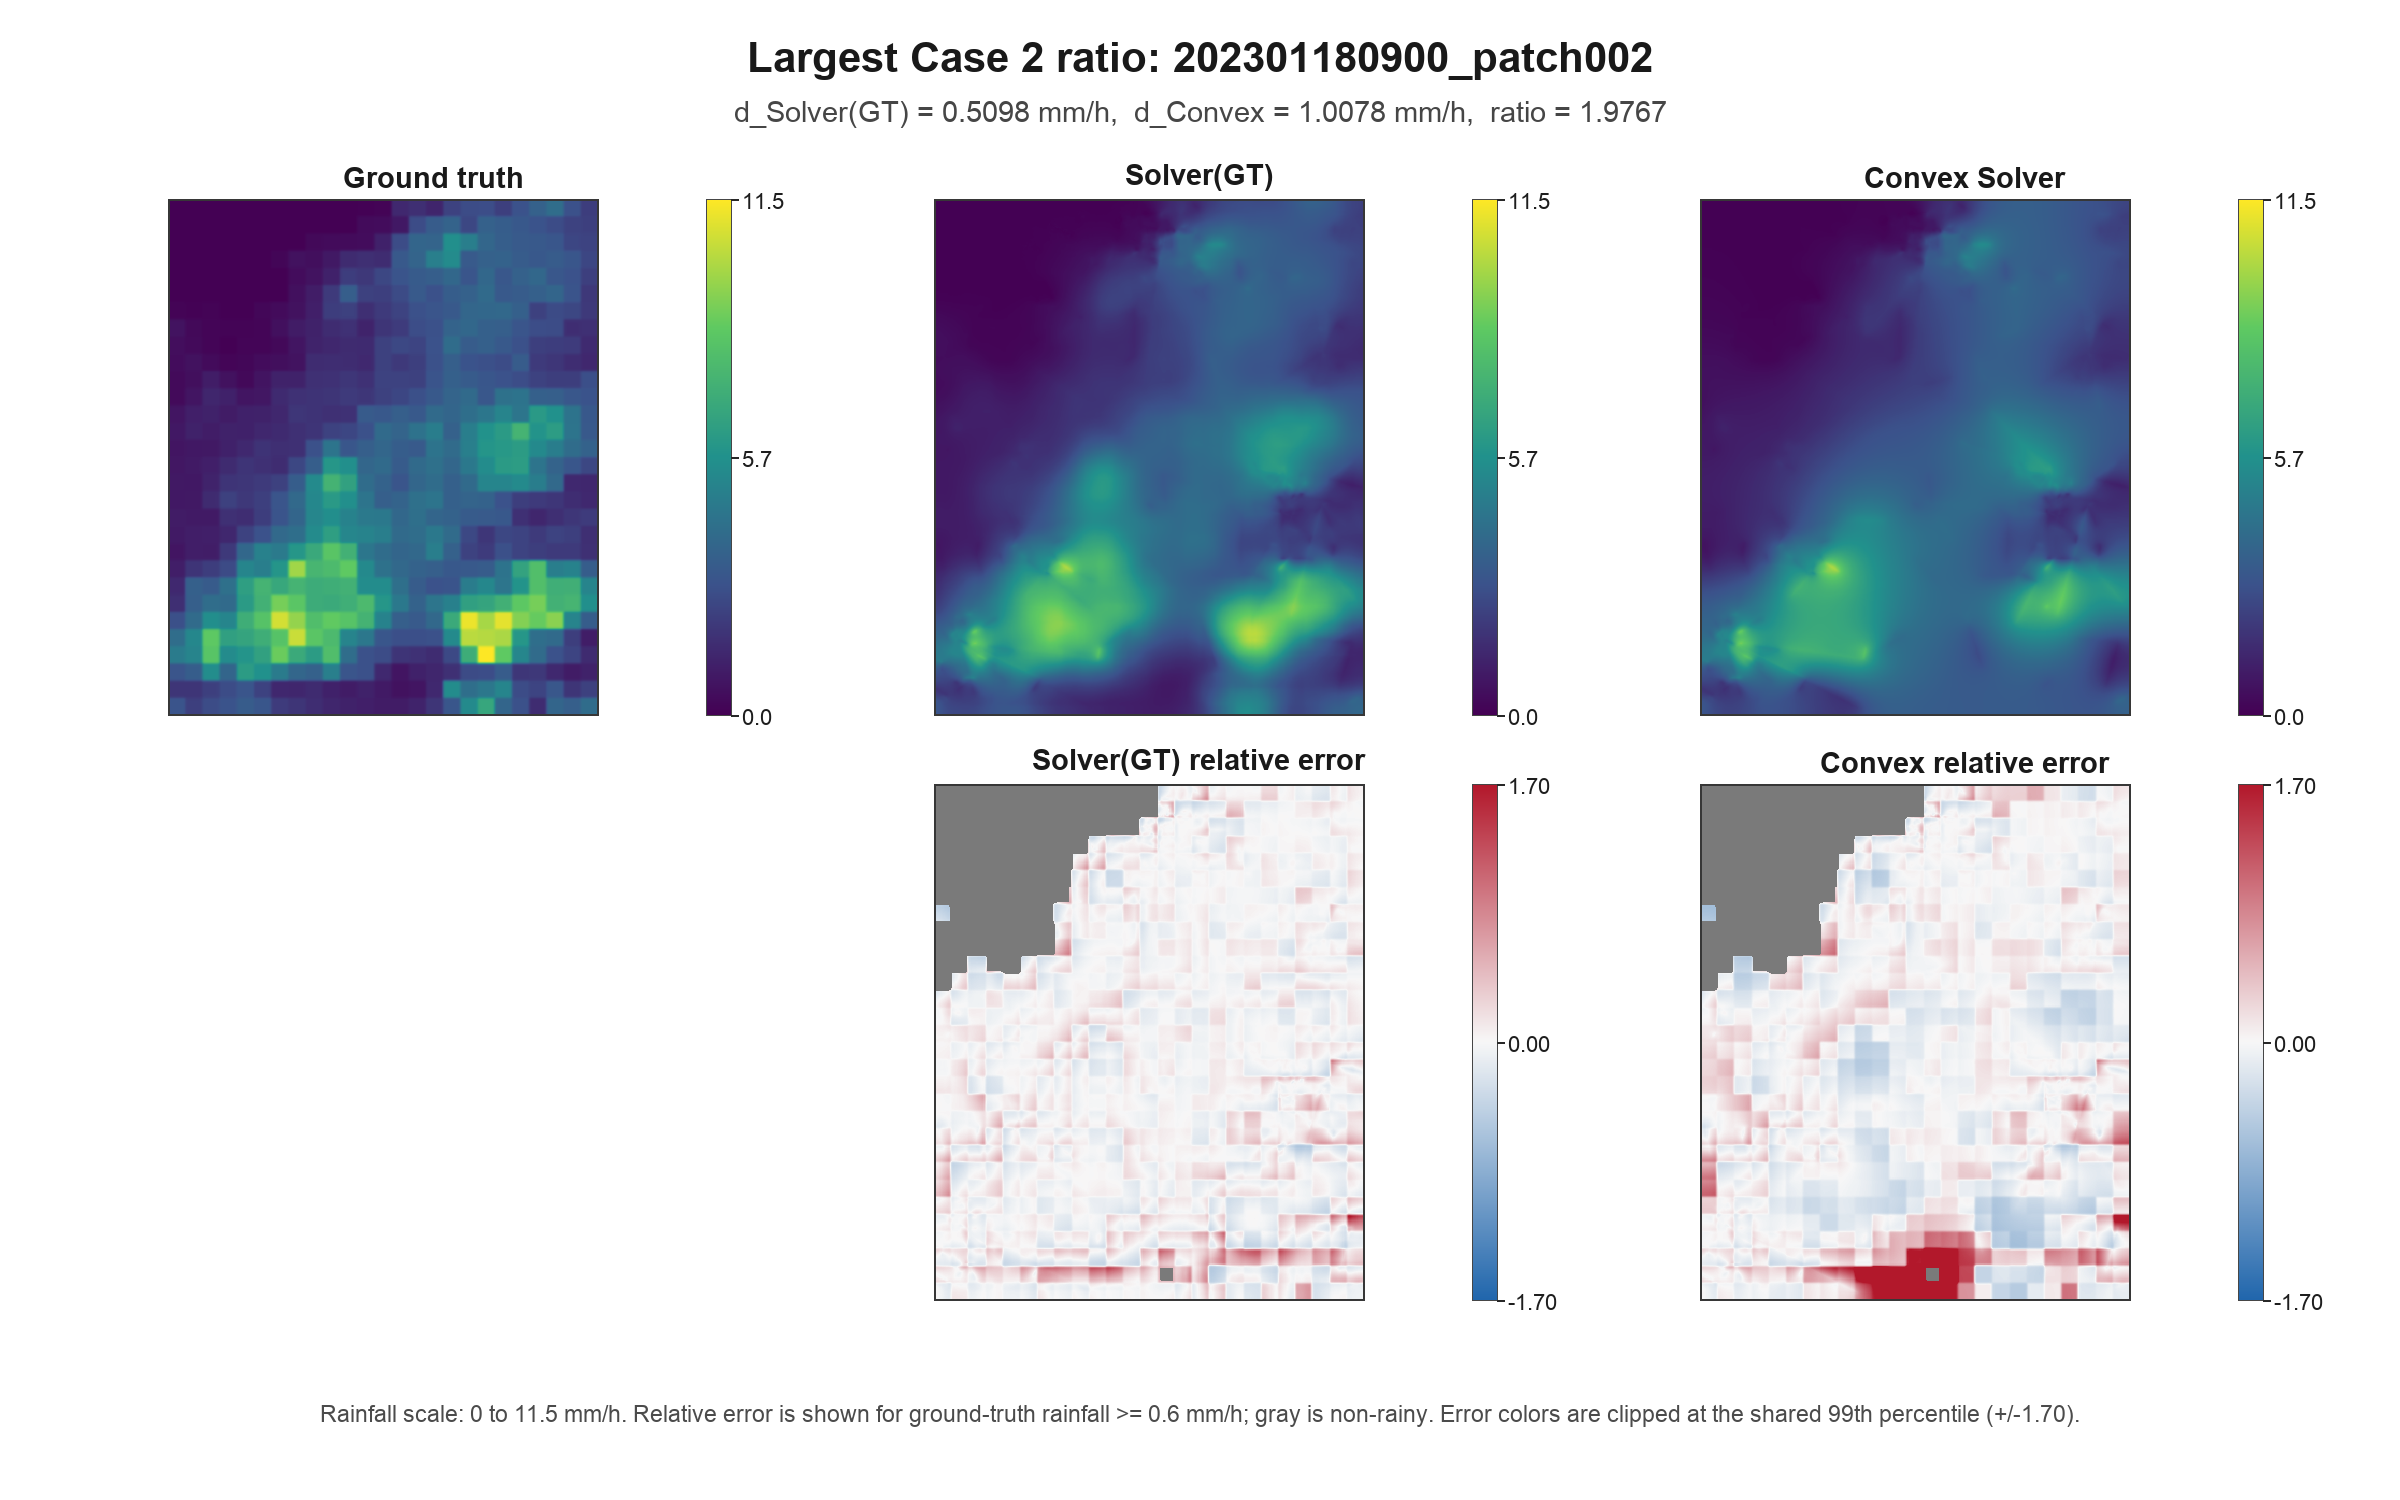
\includegraphics[width=\textwidth]{figures/largest_case2_ratio_heatmaps.png}
  \caption{Largest ratio in Case 2: \texttt{\detokenize{202301180900_patch002}}. Here $d_{\solverGT}=0.5098$~mm/h, $d_{\solverConvex}=1.0078$~mm/h, and $q=1.9767<2$.}
  \label{fig:largest-case2-ratio}
\end{figure}

\begin{figure}[H]
  \centering
  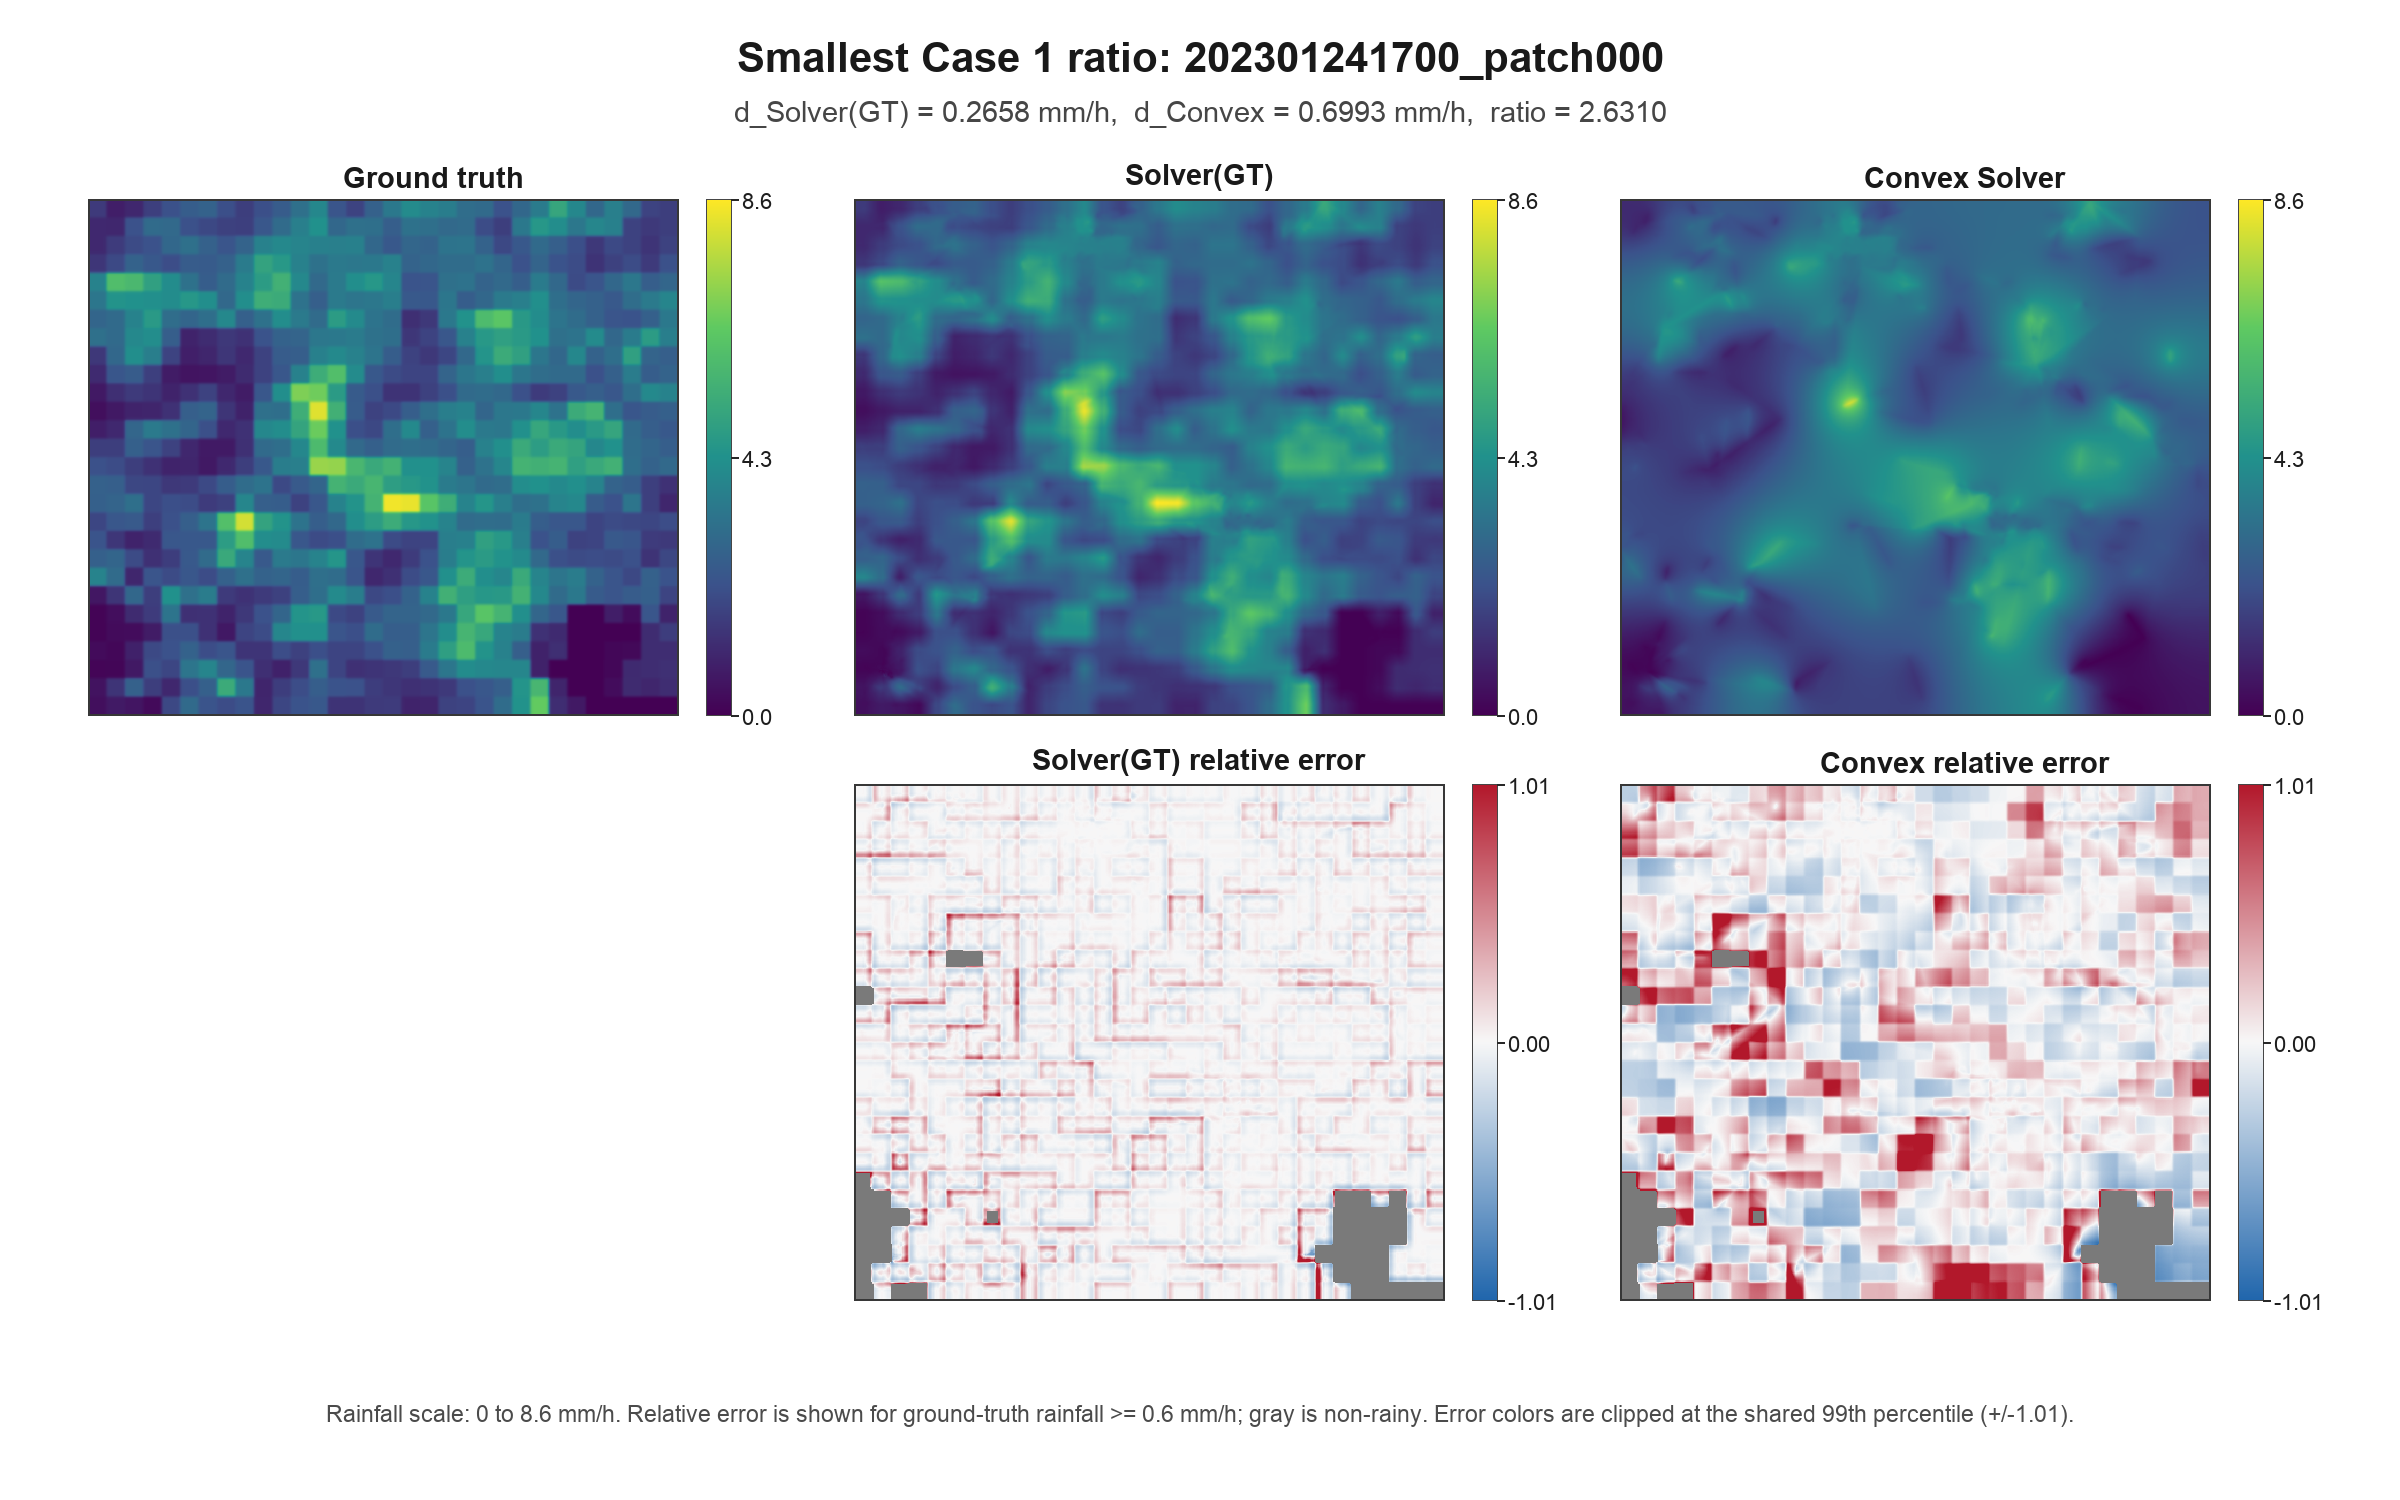
\includegraphics[width=\textwidth]{figures/smallest_case1_ratio_heatmaps.png}
  \caption{Smallest ratio in Case 1: \texttt{\detokenize{202301241700_patch000}}. Here $d_{\solverGT}=0.2658$~mm/h, $d_{\solverConvex}=0.6993$~mm/h, and $q=2.6310\geq 2$.}
  \label{fig:smallest-case1-ratio}
\end{figure}

\end{document}
